%%%%%%%%%%%%% PROPERTIES %%%%%%%%%%%%%
\documentclass[12pt,titlepage]{article}

%% LINESPACING %%
\usepackage{setspace}
%\doublespacing
%\singlespacing
%\onehalfspacing

%% PACKAGES %%
\usepackage{enumitem} %enumerate
\usepackage{amsmath}  %maths typsetting
\usepackage{amssymb}  %extra AMS symbols
\usepackage{graphicx} %extra image options
\usepackage{float}    %float numbers
\usepackage{cite}     %citation handling
\usepackage{lipsum}   %automatically generate text
\usepackage{caption}  %caption handling
\usepackage{microtype}%improves general appearance
\usepackage{hyperref} %use hyperlinks
\usepackage{wrapfig}  %similar to MSword wrap text
\usepackage{courier}  %courier text (used for code)
\usepackage{indentfirst} %indent the firsts paragraphs
\usepackage[para,symbol*]{footmisc} 
%puts footnotes on the same line and enables the use of symbols

%% PAGE MARGINS %%
\oddsidemargin  0.0in
\evensidemargin 0.0in
\textwidth      16cm  % gives approx 1-inch right margin
\headheight     0.0in
\topmargin      0.0in
\textheight     22cm
\renewcommand{\topfraction}{0.9}
\renewcommand{\bottomfraction}{0.0}
\renewcommand{\textfraction}{0.1}
\renewcommand{\floatpagefraction}{0.9}

%% EXTRA %%
% no gaps between enumerations
\setlist[itemize]{noitemsep, topsep=0pt} 
% enables the use of '\tab' command
\newcommand\tab[1][1cm]{\hspace*{#1}}   

\hypersetup{colorlinks,urlcolor=blue}

%%%%%%%%%%%%%%%%%%%%%%%%%%%%%%%%%%%%%%%%%%%%%%%%%%%%%

\begin{document}

% set numbering
\pagenumbering{arabic}
\setcounter{page}{1}		

%% MINI COVER AND AUTHORS %%
\begin{center}
	\line(1,0){300} \\
	[0.10in]
	\huge{\bfseries Technical Report} \\
	[0.2in]
	\large{\bfseries Detailed classification of swimming paths in the Morris Water Maze: multiple strategies within one trial
		\footnote[1]{\textit{Gehring, T. V., Luksys, G., Sandi, C., and Vasilaki, E. (2015) Detailed classification of swimming paths in the Morris Water Maze: multiple strategies within one trial. Scientific Reports, Nature Publishing Group, 5, 14562; doi: 10.1038/srep1456.}}}
	\\
	[0.2in]
	\Large{\bfseries Code description and reproducibility of the  results}
	\\
	[0.005in]
	\line(1,0){300} \\
\end{center}
\noindent
\large{\textbf{Avgoustinos Vouros$^1$, Tiago V. Gehring$^1$, Mike Croucher$^1$ \& Eleni Vasilaki$^1$}}
\\ \\
\noindent	
{\small$^1$ Department of Computer Science, University of Sheffield, Sheffield, UK. Correspondence and requests for materials should be addressed to E.V. (email: e.vasilaki$@$sheffield.ac.uk).}
\\

%%%%% MAIN REPORT %%%%%
\begin{doublespace}
\section{Introduction}

\indent This software can be used to analyse the trajectories of animals by means of a semi-supervised clustering algorithm.

For more details of the analysis procedure, as applied to trajectories in the Morris Water Maze, please refer to \href{http://www.nature.com/articles/srep14562}{Gehring et al., 2015}. The data used in this article is also provided here as an example application of the code. Although this code was initially applied to trajectories in the Morris Water Maze, the method is general enough as to be applied to other types of experiment.

Please note that this code works only with the specific data provided and for the experimental set up of Morris Water Maze described in the paper. A generalized and updated version is provided \href{https://github.com/RodentDataAnalytics/roda}{here}. The updated version has an improved graphical user interface and a complete description on how the code may be used with user defined experimental setups and data.


\section{Provided Functions}

This software provides the following main functionality:
\begin{itemize}
	\item A graphical user interface (GUI) for browsing and tagging trajectories or segments of trajectories (\textbf{gui$/$browse\_trajectories.m}). A secondary window, from the GUI, providing multiple data visualizations (such as individual feature values and clusters) can be accessed. The GUI can also start the semi-supervised clustering algorithm used to classify similar trajectories or segments;
	
	\item Semi-supervised clustering algorithm (\textbf{semisupervised\_clustering.m}): this class is a front end for the MPCKmeans semi-supervised algorithm. It uses manually labelled data (provided as mapping from trajectory segments to of one or more behavioural classes) to define must-link and cannot-link constraints.
	
	\item Plotting routines for plotting trajectories (\textbf{plot\_trajectory.m}) or the classification results in the form of color bars (one color for each behavioural class) for each trajectory (\textbf{plot\_distribution\_strategies.m});
	
	\item Various other functions for analyzing and validating the clustering results. These functions are inside the \textbf{results$/$mwm} folder and are used to generate the results and figures of the publication referenced above. This publication focuses on the comparison of the behaviour between stressed and non-stressed rats in the Morris Water Maze experiment.
\end{itemize}


\section{Using the Code}
\subsection{Quick Run}

In order to reproduce any of the results of the paper the file \textbf{initialize.m} needs to run. Then, by calling each of the scripts, available in the \textbf{results$/$mwm folder}, the various figures and results of the paper can be generated. For convenience, a script called \textbf{ALL\_RESULTS}, which generates all the results and figures at once, is provided. The generated figures and the results are stored inside the \textbf{results$/$generated} folder.

To activate the GUI first run the file \textbf{initialize.m} and then one of the following commands:
\begin{itemize}
	\item browse\_set(1,0): the full (i.e. non-segmented) trajectories.
	\item browse\_set(2,0): segmented swimming paths without any reference configuration.
\end{itemize}

\subsection{Generating the paper's results}

The scripts in the \textbf{results$/$mwm} folder are used to generate the results and figures of the published paper, including the supplementary material. Refer to table 1 for a complete synopsis of each script's generated result as well as its connection to the paper.

Before running any of the scripts it is mandatory to run the script \textbf{initialize.m} which is located inside the home folder (\textbf{mwm-ml-master$/$}). This script loads the WEKA library (for more information refer to ``1.4 Two-stage clustering algorithm'' description of the supplementary material of the publication), the Morris water maze configurations and adds to MATLAB path the appropriate folders.

Note that the results generated by running the scripts may have differences compared to the ones in the paper. For more information on this issue please refer to section ``Differences between current code results and paper''.

\begin{table}[H]
\centering
\caption{Result Files Description}
\label{table_result_files}
\resizebox{\linewidth}{!}{%
	%|p{7cm}|p{2cm}|p{10cm}|
\begin{tabular}{|p{7cm}|p{3cm}|p{14cm}|}
\hline
	\multicolumn{1}{|c|}{\textbf{File Name}}       & \multicolumn{1}{c|}{\textbf{Generated Result}} & \multicolumn{1}{c|}{\textbf{Description}}      
	\\\hline
	ALL\_RESULTS.m               & 
	All the results of the paper &
	This script runs all the results scripts below. Please note that the script generating figure 4 page 7 will only run if the installed version of MATLAB is 2014a or earlier.
	\\\hline
	results\_control\_stress\_speed\_latency.m    &
	Main paper page 3 figure 1                    & 
	Comparison of full trajectory metrics for two groups of animals over a set of 12 trials.                                                                                                              \\\hline
	results\_trajectory\_classification.m        & 
	Main Paper page 4 figure 2                   & 
	Example of swimming paths showing different types of behaviour.                                                
	\\\hline
	results\_strategies\_individual\_evolution.m  & 
	Main paper page 7 figure 4                    & Classification results for the 6 first trials and 12 animals from the control and stress group. Please note that this script will not run unless the installed version of MATLAB is 2014a or earlier.
	\\\hline
	results\_strategies\_distributions\_length.m  & 
	Main paper page 8 figure 5 (A-H)              & 
	Average segment lengths for each strategy adopted by stress and control group of animals for a set of 12 trials divided in 3 sessions (days).                                                         
	\\\hline
	results\_transition\_counts.m    & 
	Main paper page 8 figure 5 (I)   & 
	Number of transitions between strategies for both groups showing that stressed animals change their behaviour more often within single trials.                                                        
	\\\hline
	results\_strategy\_transition\_prob.m    & 
	Main paper page 9 table 3                & 
	Transition probabilities of strategies within trials for the control and stress group of animals.                                                                                                     \\\hline
	results\_clustering\_parameters.m    & 
	Supplementary page 3 figure 2        & 
	Impact of the number of clusters on the clustering performance for a set of 29,476 segments \&amp; percentage of the full swimming paths that are covered by at least one segment of a known class.
	\\\hline
	results\_confusion\_matrix.m  & 
	Supplementary page 6 table 1  & 
	Confusion matrix for the classification of the segments.                                                                                                                                              \\\hline
	results\_class\_weights.m     & 
	Supplementary page 8 table 2  & 
	Mean and maximum length of consecutive segments of each class for the 250 cm / 90\% overlap classification with constant weights                                                   
	\\\hline
	results\_full\_trajectories\_classification2.m & 
	Supplementary page 8 figure 4                  & 
	Results of a manual classification of complete swimming paths.                                                    
	\\\hline
	results\_calibration.m          &
	Supplementary page 13 figure 8  & 
	Calibration functions                                                                                                                                                                                 \\\hline
	results \_export\_random\_segments.m  & Extra                                 & 
	Exports 50 random segments                                                                                                                                                                            \\\hline
	results\_export\_selected\_trajectories.m & Extra                                     & 
	Exports 66 selected trajectories     
	\\\hline        
	\end{tabular}}
\end{table}

\subsection{Using the GUI}

The GUI (figure \ref{gui}) can be used to label path segments, cluster the data and visualize the clustering results.

To activate the GUI first the script \textbf{initialize.m} which is located inside the home folder (\textbf{mwm-ml-master$\textbf{/}$}) needs to run. This script loads the WEKA library (for more information refer to ``1.4 Two-stage clustering algorithm description'' of the supplementary material of the publication), the Morris water maze configurations and adds to MATLAB path the appropriate folders. Afterwards the GUI can be activated by running any of the commands below:
\begin{itemize}
	\item browse\_set(1,0): loads the full (i.e. non-segmented) trajectories.
	\item browse\_set(2,0): loads the segmented swimming paths without any reference configuration.
\end{itemize}

\begin{figure}[H]
	\begin{center}
		\includegraphics[width=1\textwidth]{gui.jpg}\\
		\caption [gui]{Graphical user interface.}\label{gui}
	\end{center}
\end{figure}

\noindent\textbf{Labels:}

Multiple labels or tags (shown to the right of each path) can be defined per trajectory. Tags are automatically saved to a file defined in the configuration file; to change the output file name where the tags are saved and define new tags (among other things) please refer to the next Section.
\\
\\
\noindent\textbf{Changing the visualization:}

The default 2x2 view layout can be changed by selecting a different number of X and Y views in the bottom right control group in the GUI. There, the main visualization and up to 2 secondary ones can also be selected (these are experiment dependent and defined in the main configuration file).
\\
\\
\noindent\textbf{Filtering and sorting segments:}

Group of segments fulfilling certain criteria (e.g. all segments that are tagged/non-tagged or which belong to a certain cluster or class) can be selected by using the group of controls found in the bottom left. Segments can also be sorted according to a specific feature or, for example, according to their distance to the cluster centroids (useful for identifying edge cases of segments falling between two behavioural classes).
\\
\\
\\
\textbf{Running the clustering algorithm:}

The clustering algorithm can be run by clicking in the 'cluster' button. Before doing so it is necessary to select a target number of clusters (done also directly in the GUI). After running, the clustering results will be automatically shown; segments of specific classes or that were wrongly classified (available if the “cross-validation” option is active) can be selected by using the filtering options.


\section{Input Data Description}

The folder \textbf{data$/$mwm\_peripubertal\_stress} contains the original Morris Water Maze trajectories of rats induced to peri-pubertal stress (PPS). The data was acquired from the Laboratory of Behavioural Genetics, EPFL. For more information about the experiments see \href{http://www.nature.com/articles/srep14562}{Gehring et al., 2015}.

Trajectories were acquired with Ethovision 3.1. A total of 3 experiments were performed, which are split into three folders: set1, set2, and set3. Specific details of each trial separately may be found inside the CSV files of the three above folders.

The data provided by the Laboratory of Behavioral Genetics needs to be calibrated. Details of the calibration are given in the supplementary information of \href{http://www.nature.com/articles/srep14562}{Gehring et al., 2015}. A ready to use calibration procedure is given in the \textbf{import$/$noldus$/$calibration$/$} directory in the root folder.  For this procedure screenshots of the trajectories need to be provided. These screenshots are the PNG files inside the screenshots folder.

Finally inside the data folder the segment\_labels and the labels\_full .csv files contain labelling data of specific trajectories for the classification process. Starting from the first column each column represents the following: experimental set, day, track, off, length and the rest are labels.

For more information about the experiment properties (platform position, radius, etc) and the data (animal groups, ids, etc) refer to the \textbf{config$/$morris\_water\_maze$/$config\_mwm.m}


\section{Code Adaptation}

In order to adapt the code to other experiments please refer to this \href{https://github.com/RodentDataAnalytics/roda}{link}, which redirects to a generalized and updated version of the code. The updated version has an improved graphical user interface and a complete description on how the code may be used with user defined experimental setups and data.


\section{Requirements}

This code requires the statistics and machine learning toolbox in addition to MATLAB itself.
It is tested and working with MATLAB versions 2013, 2014a, 2015b.


\section{Known Issues}

\begin{itemize}
	\item The function results\_strategies\_individual\_evolution.m which generates the published paper's figure 4 on page 7 cannot be generated on MATLAB version 2014b and later.
	\item The generated results may contain some dissimilarity to the ones in the paper. This difference is only quantitative and is caused because fewer labels were used during the classification process when the paper was written. 
\end{itemize}


\section{Differences between current code results and paper}
The user should note that there are differences between the software's results and the results of the published paper. These changes are only quantitative and are caused due to improving the labelling quality of the data after the paper was published. Nevertheless, the results and the conclusions remain qualitatively the same.

Below there is a list of the exact results that this software produces by running the scripts inside the \textbf{results$/$mwm} folder.\\

\begin{itemize}
\item \textbf{results\_control\_stress\_speed\_latency.m}\\
(paper page 3, figure 1)
\begin{figure}[H]
	\begin{center}
		\includegraphics[width=1\textwidth]{f1.jpg}\\
		\label{code_fig1}
	\end{center}
\end{figure}
\item \textbf{results\_strategies\_individual\_evolution.m}\\
(paper page 7, figure 4)\\
The first figure refers to the controlled group while the second to the stressed group. Note that in the paper only 12 animals from each group were selected. Also the ``Direct Finding'' strategy (which means that the animal managed to find the platform directly) was removed from the paper.
\begin{figure}[H]
	\begin{center}
		\includegraphics[width=1\textwidth]{f4.jpg}\\
		\label{code_fig4}
	\end{center}
\end{figure}
\begin{figure}[H]
	\begin{center}
		\includegraphics[width=0.6\textwidth]{f4l.jpg}\\
		\label{code_fig4l}
	\end{center}
\end{figure}
\item \textbf{results\_control\_stress\_speed\_latency.m \& results\_transition\_counts.m}\\
(paper page 8, figure 5)
\begin{figure}[H]
	\begin{center}
		\includegraphics[width=1\textwidth]{f5.jpg}\\
		\label{code_fig5}
	\end{center}
\end{figure}
\item \textbf{results\_strategy\_transition\_prob.m}\\
(paper page 9, table 3)
\begin{figure}[H]
	\begin{center}
		\includegraphics[width=1\textwidth]{t3.jpg}\\
		\label{code_table3}
	\end{center}
\end{figure}
\item \textbf{results\_clustering\_parameters.m}\\
(supplementary page 3, figure 2)	
\begin{figure}[H]
	\begin{center}
		\includegraphics[width=1\textwidth]{sfig2.jpg}
		\label{code_sfig2}
	\end{center}
\end{figure}
\item \textbf{results\_confusion\_matrix.m}\\
(supplementary page 6, table 1)
\begin{figure}[H]
	\begin{center}
		\includegraphics[width=1\textwidth]{st1.jpg}\\
		\label{code_stable1}
	\end{center}
\end{figure}
\item \textbf{results\_class\_weights.m}
(supplementary page 8, table 2)
\begin{figure}[H]
	\begin{center}
		\includegraphics[width=1\textwidth]{st2.jpg}\\
		\label{code_stable2}
	\end{center}
\end{figure}
\item \textbf{results\_full\_trajectories\_classification2.m}\\
(supplementary page 8, figure 4)
\begin{figure}[H]
	\begin{center}
		\includegraphics[width=1\textwidth]{sf4.jpg}\\
		\label{code_sfig4}
	\end{center}
\end{figure}
\item \textbf{results\_calibration.m}\\
(supplementary page 13, figure 8 and page 14, figure 10)
\begin{figure}[H]
	\begin{center}
		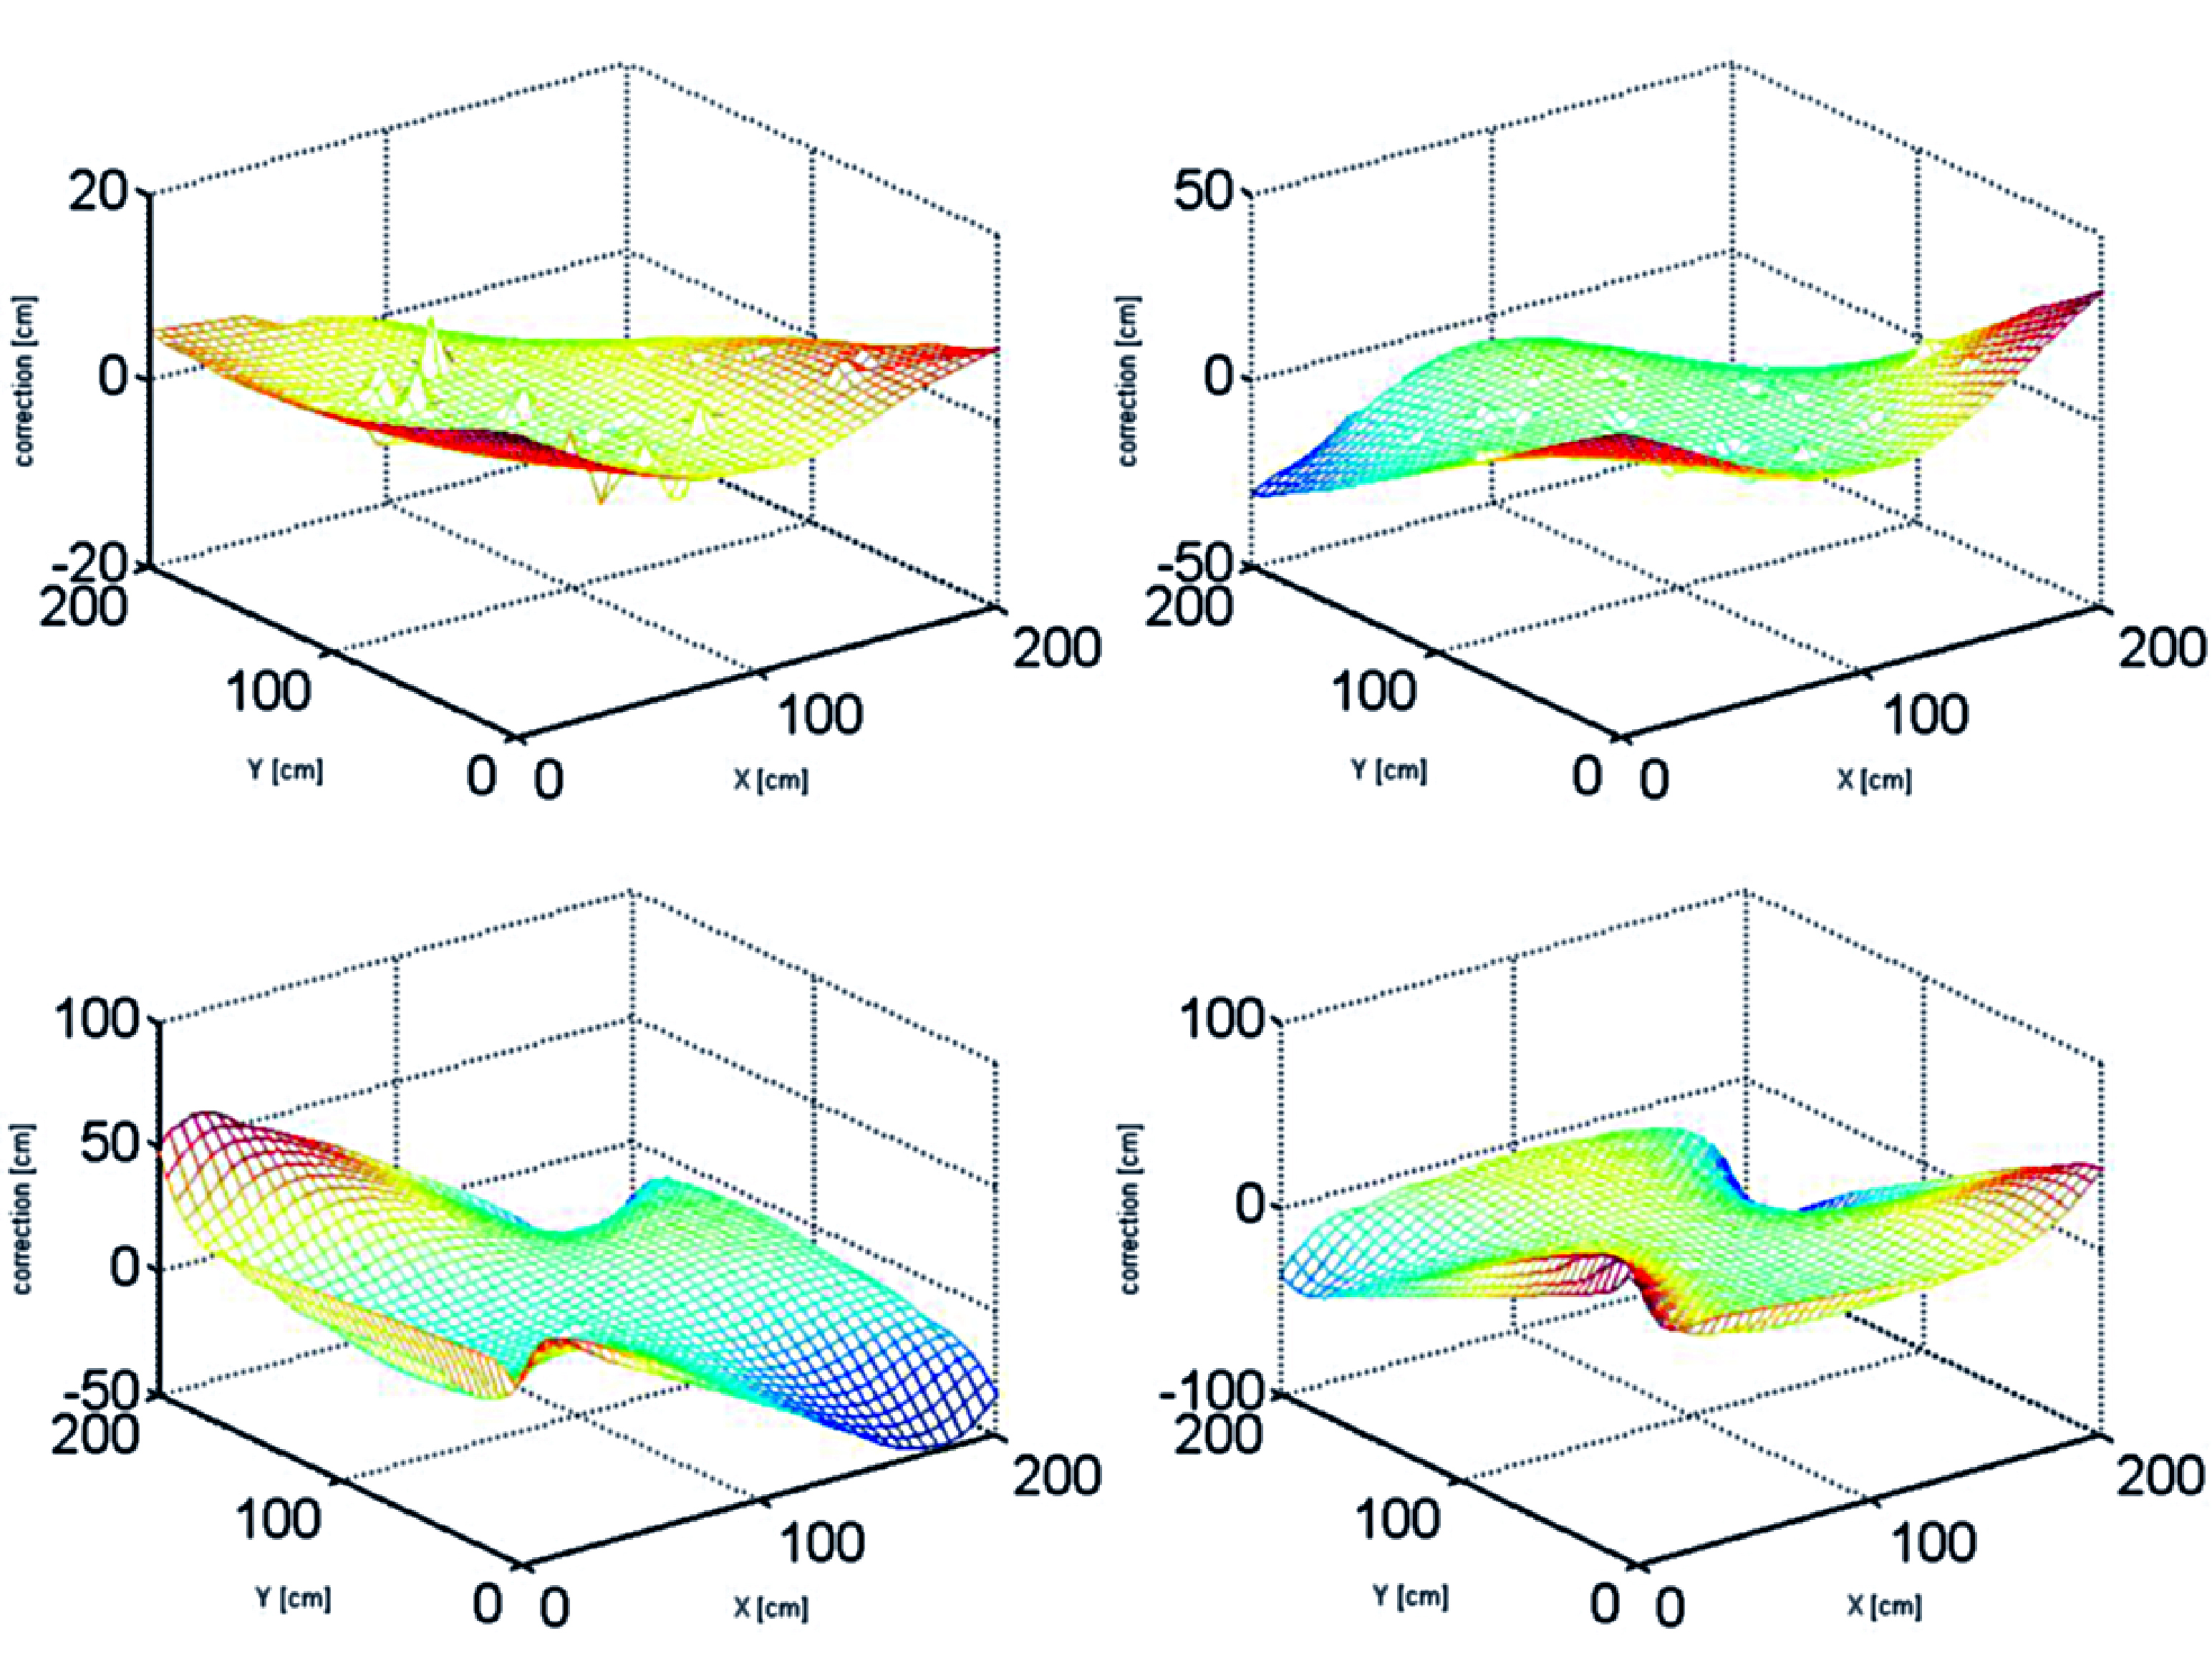
\includegraphics[width=1\textwidth]{sf8.jpg}\\
		\label{code_sfig8}
	\end{center}
\end{figure}
\begin{figure}[H]
	\begin{center}
		\includegraphics[width=0.5\textwidth]{sf10.jpg}\\
		\label{code_sfig10}
	\end{center}
\end{figure}

\end{itemize}


\section{In-depth Code Explanation}

\subsection{Configurations}
Inside the \textbf{config} folder are the configuration files of the software.

The \textbf{base\_config.m} is used as the base configuration upon which other configuration files for specific experiments and experimental setups can be build. The \textbf{config\_mwm.m} contains the configurations of the specific Morris Water Maze experimental setup which was used for the publication of \href{http://www.nature.com/articles/srep14562}{Gehring et al., 2015}.

As mentioned in the Code Adaptation section, the current code is linked to the specific Morris Water Maze setup described in the publication above. Thus, in order to adapt the code to other experiments please refer to this \href{https://github.com/RodentDataAnalytics/roda}{link}

\subsection{Data Representation}
The scripts inside the folder \textbf{data\_representation} among with trajectory\_simplify\_implementation.m are called to compute values along the trajectories (e.g. speed) or to change the coordinate system.

\subsection{Utility}
The \textbf{utility} folder contains scripts for the generation of hash values. Hash values are used throughout the code and assigned to trajectories, segments of trajectories, classification process, etc in order to boost the running speed of the software.

\subsection{The Noldus Functions}

\textbf{import$/$noldus$/$}\linebreak
\tab load\_calibration\_data.m\linebreak
\tab load\_trajectories.m\linebreak
\textbf{\tab calibration$/$}\linebreak
\tab\tab calibrate\_trajectory.m\linebreak
\tab\tab read\_ethovision.m\linebreak
\tab\tab read\_trajectory.m\linebreak
\tab\tab trajectory\_calibration\_data.m\linebreak
\tab\tab trajectory\_points\_from\_snapshots.m\linebreak
\tab\tab trajectory\_snapshot\_position.m\linebreak

The Noldus functions inside the import folder are responsible for parsing various information from CSV data files, created by Ethovision 3.1. The collaboration of these function is shown in figure \ref{noldus}.

\begin{figure}[H]
	\begin{center}
		\includegraphics[width=1\textwidth]{noldus.jpg}\\
		\caption [noldus]{Noldus flowchart.}\label{noldus}
	\end{center}
\end{figure}

\begin{itemize}
	\item\textbf{load\_trajectories.m:}
	 Imports trajectories from set(1...N) folders inside \textit{data$/$mwm\_peripubertal\_stress$/$}
	\item\textbf{load\_calibration\_data.m:}
	 Loads calibrated data if available else calibrates raw data and load them.
	\item\textbf{trajectory\_points\_from\_snapshots:}
	 Processes a directory with a series of trajectory snapshots. Returns a list of time and coordinates for this trajectory.
	\item\textbf{trajectory\_snapshot\_position:}
	 Extracts position from snapshots located inside  \textit{data$/$mwm\_peripubertal\_stress$/$screenshots$/$set(1...N)$/$}
	\item\textbf{read\_trajectory.m:}
	 Parses various information about the animals and their trajectories. Calls \textbf{read\_ethovision.m} which reads a trajectory from a CSV data file created by Ethovision 3.1.
\end{itemize}

\subsection{The features Scripts}
The folder \textbf{features} contains scripts for the calculation of the segments' features. For more information about each feature refer to the main paper, page 10, section ``Methods''.

\subsection{The Graphical User Interface}
The 'gui' folder contains the code which builds the graphical user interface. As the GUI is used mainly for visualisation purposes, the reader may refer to the section Result Files for a complete review of the background processes.

\subsection{Results}
Inside the \textbf{results$/$mwm} folder there are scripts that generate the results and figures of the publication \href{http://www.nature.com/articles/srep14562}{Gehring et al., 2015}. The flowchart of each of these files can be found in the subsections below. Note the \textbf{export\_figure.m} is only used for exporting the generated figures and does not generate any results. 

The results of the scripts are stored inside the \textbf{results$/$generated} folder. The already generated file \textbf{calibration\_data\_123.mat} contains the correct trajectories after the calibration process.

Running the various result scripts will lead to the generation of the \textbf{cache} folder which will contain the files \textbf{features\_values.mat} and \textbf{trajectories\_\%id.mat}. The first file contains the calculated features and the second one all the trajectories (\%id refers to a unique generated number, for this program the generated one is 1147731521). 

\subsubsection{results\_control\_stress\_speed\_latency.m}
Comparison of full trajectory metrics for two groups of animals over a set of 12 trials (produces: paper page 3, figure 1).

\begin{figure}[H]
	\begin{center}
		\includegraphics[width=0.99\textwidth]{results_control_stress_speed_latency.jpg}
		\label{fig1}
	\end{center}
\end{figure}

\begin{itemize}
	\item\textbf{initialize global variables:} loads the Morris water maze configurations and initializes the global variables below:\\
	 (a) \textit{g\_trajectories\_speed:} movement speed.\\
	 (b) \textit{g\_trajectories\_length:} path length.\\
	 (c) \textit{g\_animals\_trajectories\_map:} matrix of trajectory indices for each trial and group of animals.\\
	 (d) \textit{g\_trajectories:} total trajectories (only for two animal groups, controlled and stressed)
	\item\textbf{cache\_animals:} calculates or loads (if already exist) the data of the global variables above.
	\item\textbf{check significances:} uses the external function sigstar \href{http://www.mathworks.com/matlabcentral/fileexchange/39696-sigstar-groups-stats-nosort-}{(Rob Campbell, 2013)} to add significance stars and lines highlighting significant differences between pairs of groups.
	\item\textbf{export\_figure:} exports the current figure in EPS and FIG format (default).
\end{itemize}

\subsubsection{results\_trajectory\_classification.m}
Runs the classification process twice for 15 trajectories: (a) once using a mapping with constant weight (see generated files ending with ``\_cons'' inside the \textbf{results$/$generated} folder, (b) once using different weights per class. The generated file \textbf{strategies\_line\_legend\_vert} contains the legend of the figures (produces: paper page 4, figure 2).

\begin{figure}[H]
	\begin{center}
		\includegraphics[width=0.6\textwidth]{results_trajectory_classification.jpg}
		\label{fig2}
	\end{center}
\end{figure}

\begin{itemize}
	\item\textbf{initialize global variables:} loads the Morris water maze configurations and initializes the global variables below:\\
	(a) \textit{g\_trajectories:} total trajectories.\\
	(b) \textit{g\_segments:} total segments produced from the splitting of trajectories.\\
	(c) \textit{g\_segments\_classification:} classification of segments (splited trajectories).\\
	(d) \textit{g\_segments\_base\_classification:} classification data of all segments.\\
	(e) \textit{g\_long\_trajectories\_map:} matrix of trajectory indices for each trial and group of animals.\\
	(f) \textit{g\_partitions:} number of instances of the same trajectory class.
	\item\textbf{cache\_trajectories\_classification:}  calculates the data of the global variables above.
	\item\textbf{export\_figure:} exports the current figure in EPS and FIG format (default).
\end{itemize}

\subsubsection{results\_strategies\_individual\_evolution.m}
Classification results for each trial and 27 animals from the control and stress group. The generated figures show the changes in exploration strategies of the animals over the trials. Note that in order to export the generated figures the code line 74:\\
\noindent\fbox{%
 \parbox{\textwidth}{%
  \small{\texttt{\%export\_figure(1,gcf,g\_config.OUTPUT\_DIR,\\ \tab\tab sprintf('individual\_strategies\_g\%d\_s\%d',g,s));}}
 }%
}\\
needs to be uncommented (remove the \% character). The exporting process requires an extensive amount of time. (produces: paper page 7 figure 4). 

\begin{figure}[H]
	\begin{center}
		\includegraphics[width=0.6\textwidth]{results_strategies_individual_evolution.jpg}
		\label{fig4}
	\end{center}
\end{figure}

\begin{itemize}
	\item\textbf{initialize global variables:} loads the Morris water maze configurations and initializes the global variables below:\\
	(a) \textit{g\_segments\_classification:} classification of segments (splited trajectories).\\
	(b) \textit{g\_partitions:} number of instances of the same trajectory class.\\
	(c) \textit{g\_animals\_ids:} animal ids (controlled and streessed groups).\\
	(d) \textit{g\_animals\_trajectories\_map:} matrix of trajectory indices for each trial and group of animals.
	\item\textbf{cache\_animals:} calculates or loads (if already exist) the data of the global variables \textit{g\_animals\_trajectories\_map} and \textit{g\_animals\_ids}.
	\item\textbf{cache\_trajectories\_classification:}  calculates the data of the global variables \textit{g\_segments\_classification} and \textit{g\_partitions}.
\end{itemize}

\subsubsection{results\_strategies\_distributions\_length.m}
Average length in meters that animals spent in each one strategy, for a total of 8 strategies, during each trial (produces: paper page 8, figure 5 [A-H]).

\begin{figure}[H]
	\begin{center}
		\includegraphics[width=0.8\textwidth]{results_strategies_distributions_length.jpg}
		\label{fig5}
	\end{center}
\end{figure}

\begin{itemize}
	\item\textbf{initialize global variables:} loads the Morris water maze configurations and initializes the global variables below:\\
	(a) \textit{g\_segments\_classification:} classification of segments (splited trajectories).\\
	(b) \textit{g\_animals\_trajectories\_map:} matrix of trajectory indices for each trial and group of animals.\\
	(c) \textit{g\_long\_trajectories\_map:} Through the segmentation process some trajectory segments may end with illogical length (length $=$ 0). This variable holds  indication of the ones with length $>$ 0 only.
	\item\textbf{cache\_animals:} calculates or loads (if already exist) the data of the global variable \textit{g\_animals\_trajectories\_map}.
	\item\textbf{cache\_trajectories\_classification:}  calculates the data of the global variables \textit{g\_long\_trajectories\_map} and \textit{g\_segments\_classification}.
	\item\textbf{export\_figure:} exports the current figure in EPS and FIG format (default).
\end{itemize}


\subsubsection{results\_transition\_counts.m}
Number of transitions between
strategies for both groups (produces: paper page 8, figure 5 [I]).

\begin{figure}[H]
	\begin{center}
		\includegraphics[width=0.7\textwidth]{results_transition_counts.jpg}
		\label{fig5i}
	\end{center}
\end{figure}

\begin{itemize}
	\item\textbf{initialize global variables:} loads the Morris water maze configurations and initializes the global variables below:\\
	(a) \textit{g\_segments\_classification:} classification of segments (splited trajectories).\\
	(b) \textit{g\_trajectories:} total trajectories (only for two animal groups, controlled and stressed).\\
	(c) \textit{g\_segments:} total segments produced from the splitting of trajectories.
	\item\textbf{cache\_trajectories\_classification:}  calculates the data of the global variables g\_long\_trajectories\_map and g\_segments\_classification.
	\item\textbf{export\_figure:} exports the current figure in EPS and FIG format (default).
\end{itemize}

\subsubsection{results\_strategy\_transition\_prob.m}
Transition probabilities of strategies within trials for the control and stress group of animals (produces: paper page 9, table 3).

\begin{figure}[H]
	\begin{center}
		\includegraphics[width=0.5\textwidth]{diagram_strategy_transition_prob.jpg}
		\label{table3}
	\end{center}
\end{figure}

\begin{itemize}
	\item\textbf{initialize global variables:} loads the Morris water maze configurations and initializes the global variables below:\\
	(a) \textit{g\_segments\_classification:} classification of segments (splited trajectories).\\
	(b) \textit{g\_trajectories:} total trajectories (only for two animal groups, controlled and stressed).\\
	(c) \textit{g\_long\_trajectories\_map:} Through the segmentation process some trajectory segments may end with illogical length (length $=$ 0). This variable holds  indication of the ones with length $>$ 0 only.\\
	(d) \textit{g\_partitions:} Number of instances of the same trajectory class.\\
	(e) \textit{g\_trajectories\_group:} In which animal group each trajectory belongs to (group number is specified in the configuration file).
	\item\textbf{cache\_trajectories\_classification:}  calculates the data of the global variables above.
\end{itemize}

\subsubsection{results\_clustering\_parameters.m}
Shows the impact of the number of clusters on the clustering performance for a set of 29,476 segments (produces: supplementary page 3, figure 2).

\begin{figure}[H]
	\begin{center}
		\includegraphics[width=0.5\textwidth]{results_clustering_parameters.jpg}
		\label{sfig2}
	\end{center}
\end{figure}

\begin{itemize}
	\item\textbf{initialize global variables:} loads the Morris water maze configurations and initializes the global variable below:\\
	(a) \textit{g\_segments:} total segments produced from the splitting of trajectories.
	\item\textbf{cache\_trajectory\_segments:} Loads trajectories if not already loaded and segmented them using the default segmentation parameters as defined in the global constants.
	\item\textbf{export\_figure:} exports the current figure in EPS and FIG format (default).
\end{itemize}

\subsubsection{results\_confusion\_matrix.m}
Computes the confusion matrix for the classification of segments (produces: supplementary page 6, table 1).

\begin{figure}[H]
	\begin{center}
		\includegraphics[width=0.6\textwidth]{results_confusion_matrix.jpg}
		\label{stable1}
	\end{center}
\end{figure}

\begin{itemize}
	\item\textbf{initialize global variables:} loads the Morris water maze configurations and initializes the global variable below:\\
	(a) \textit{g\_segments:} total segments produced from the splitting of trajectories.
	\item\textbf{cache\_trajectory\_segments:} Loads trajectories if not already loaded and segmented them using the default segmentation parameters as defined in the global constants.
\end{itemize}

\subsubsection{results\_class\_weights.m}
Produces the Mean and Maximum Length of consecutive segments of each class for the 250 cm $/$ 90\% overlap classification with constant weights and after adopting differentiated weights for minor and major classes (produces: supplementary page 8 table 2).

\begin{figure}[H]
	\begin{center}
		\includegraphics[width=0.6\textwidth]{results_class_weights.jpg}
		\label{stable2}
	\end{center}
\end{figure}

\begin{itemize}
	\item\textbf{initialize global variables:} loads the Morris water maze configurations and initializes the global variable below:\\
	(a) \textit{g\_segments\_base\_classification:} classification data of all segments.
	\item\textbf{cache\_trajectories\_classification:}  calculates the data of the global variables above.
\end{itemize}
	
\subsubsection{results\_full\_trajectories\_classification2.m}
Results of manual classification of complete swimming paths for all the behavioural classes (produces: supplementary page 8 figure 4).

\begin{figure}[H]
	\begin{center}
		\includegraphics[width=0.6\textwidth]{results_full_trajectories_classification2.jpg}
		\label{sfig4}
	\end{center}
\end{figure}

\begin{itemize}
	\item\textbf{initialize global variables:} loads the Morris water maze configurations and initializes the global variable below:\\
	(a) \textit{g\_trajectories:} total trajectories (only for two animal groups, controlled and stressed).\\
	(b) \textit{g\_long\_trajectories\_map:} Through the segmentation process some trajectory segments may end with illogical length (length $=$ 0). This variable holds  indication of the ones with length $>$ 0 only.\\
	(c) \textit{g\_animals\_trajectories\_map:} matrix of trajectory indices for each trial and group of animals.
	\item\textbf{cache\_animals:} calculates or loads (if already exist) the data of the global variable g\_animals\_trajectories\_map.
	\item\textbf{cache\_trajectory\_segments:} Loads trajectories if not already loaded and segmented them using the default segmentation parameters as defined in the global constants.
	\item\textbf{export\_figure:} exports the current figure in EPS and FIG format (default).
\end{itemize}

\subsubsection{results\_calibration.m}
Produces the calibration functions (x and y axis correction) and the calibration error of the three sets (produces: supplementary page 13 figure 8).

\begin{figure}[H]
	\begin{center}
		\includegraphics[width=0.5\textwidth]{results_calibration.jpg}
		\label{sfig8-10}
	\end{center}
\end{figure}

\begin{itemize}
	\item\textbf{load\_trajectories:} refer to Noldus Functions.
	\item\textbf{export\_figure:} exports the current figure in EPS and FIG format (default).
\end{itemize}	

\subsubsection{results\_export\_random\_segments.m}
Exports 50 random segments.

\begin{figure}[H]
	\begin{center}
		\includegraphics[width=0.5\textwidth]{results_export_random_segments.jpg}
		\label{rand_seg}
	\end{center}
\end{figure}

\begin{itemize}
	\item\textbf{initialize global variables:} Initializes the global variable below:\\
	(a) \textit{g\_segments:} total segments produced from the splitting of trajectories.
	\item\textbf{cache\_trajectory\_segments:} Loads trajectories if not already loaded and segmented them using the default segmentation parameters as defined in the global constants.
\end{itemize}	

\subsubsection{results\_export\_selected\_trajectories.m}
Exports some trajectories of interest

\begin{figure}[H]
	\begin{center}
		\includegraphics[width=0.5\textwidth]{results_export_selected_trajectories.jpg}
		\label{selected_traj}
	\end{center}
\end{figure}

\begin{itemize}
	\item\textbf{initialize global variables:} Loads the Morris water maze configurations and initializes the global variable below:\\
	(a) \textit{g\_segments:} total segments produced from the splitting of trajectories.\\
	(b) \textit{g\_trajectories:} total trajectories (only for two animal groups, controlled and stressed).\\
	(c) \textit{g\_long\_trajectories\_map:} Through the segmentation process some trajectory segments may end with illogical length (length $=$ 0). This variable holds  indication of the ones with length $>$ 0 only.
	\item\textbf{cache\_trajectory\_segments:} Loads trajectories if not already loaded and segmented them using the default segmentation parameters as defined in the global constants.
\end{itemize}	

\section*{Acknowledgements}
We would like to thank Nikos Gkaniaris for his thorough reading of this document.


\end{doublespace}
	
\end{document}	
